\documentclass[xcolor=dvipsnames,xcolor=table]{beamer} % dvipsnames gives more built-in\\
\usetheme{Madrid}
\usepackage[spanish,es-tabla]{babel}
\hypersetup{pdfpagemode=FullScreen}
\usepackage{ragged2e}
\usepackage{etoolbox}
\usepackage{bbding}
\apptocmd{\frame}{}{\justifying}{} % Allow optional arguments after frame.\textbf{}
%\useoutertheme{miniframes} % Alternatively: miniframes, infolines, split
\useinnertheme{circles}
\definecolor{UBCblue}{rgb}{0.04706, 0.13725, 0.26667} % UBC Blue (primary)
\usecolortheme[named=UBCblue]{structure}
%---------------TITULO--------------------------------------------
\title[Diagnóstico del cáncer de mama]{Metodología para la aplicación de la ciencia de datos en el diagnóstico del cáncer de mama}
\author[Jorge M., Edith A.]{Presenta:\\ Esp.Jorge Armando Millán Gómez}
\institute[Universidad Distrital]{Universidad Distrital ``Francisco José de Caldas''\\Maestria en ciencias de la información y las comunicaciones}
\date{\today}
\logo{
\includegraphics[height=1.5cm]{PROYECTO/imgs/LogoUdistrital}}

%---------------INICIO--------------------------------------------
\begin{document}

%----------------FRAME---------------------------------------------------------------
\begin{frame}
	\titlepage
\end{frame}
%----------------FRAME--------------------------------------------------------------
\begin{frame}
	\frametitle{Elementos principales de la investigación}
	\begin{block}{Planteamiento del Problema}\justifying
	Según el informe de la organización mundial de la salud del año 2020 los casos detectados de cáncer de mama en Colombia fueron 15.509 de los cuales 4.411 casos terminaron en muerte ocupando el primer puesto de la tasa de letalidad sobre los demás tipos de cáncer\cite{InternationalAgencyforResearchonCancer2020}. Si no se tiene un diagnóstico a tiempo que detecte los aspectos más significativos que caracterizan el cáncer de mama es posible que la cifra de muertes en Colombia sea mayor en los años posteriores. En consecuencia, es necesario desarrollar una metodología que facilite la aplicación de la ciencia de datos en el diagnóstico de esta enfermedad.
	\end{block}
\end{frame}

%----------------FRAME--------------------------------------------------------------
\begin{frame}
	\frametitle{Elementos principales de la investigación}
	\begin{block}{Formulación del Problema}\justifying
		\begin{itemize}
		 	\item ¿Una metodología aplicada a técnicas en ciencias de datos para el diagnóstico de cáncer de mama mejora y facilita el análisis de patrones característicos en cada individuo para encontrar errores en el diagnostico? 
		\end{itemize}
	\end{block}
\end{frame}


%----------------FRAME--------------------------------------------------------------
\begin{frame}
	\frametitle{Elementos principales de la investigación}
	\begin{block}{Planteamiento de la Hipótesis} \justifying
	\begin{itemize}
		\item Una metodología para comparar técnicas y grandes cantidades de datos que contienen información de resultados diagnósticos de pacientes particulares con los datos característicos de pacientes que padecen de cáncer de mama, permite hallar la similitud del comportamiento de los datos y predice de manera correcta el padecimiento de este tipo de cáncer de los pacientes particulares e identifica las variables que más influyen para contraer dicha enfermedad. 
	\end{itemize}

	\end{block}
\end{frame}
%----------------FRAME--------------------------------------------------------------
\begin{frame}
	\frametitle{Objetivos}
	\begin{block}{Objetivo General}
		\justifying		
		Desarrollar un sistema con modelos de Machine Learning para diagnosticar el padecimiento de cáncer de mama.
	\end{block}
	
	\begin{alertblock}{Resultado}
		\justifying	
		Desarrollo de una aplicación web para el diagnóstico del cáncer de mama donde se utilizaron modelos de Machine Learning seleccionados a partir de la exploración y comparación de los modelos más utilizados por diferentes investigadores y la precisión de dichos modelos  en el diagnóstico de este tipo de Cáncer. 
	\end{alertblock}

\end{frame}

%----------------FRAME--------------------------------------------------------------
\begin{frame}
	\frametitle{Objetivos}
	\begin{block}{Objetivos Especificos}\justifying
		Efectuar el entrenamiento de los modelos en Machine Learning que apliquen para el diagnostico de cáncer de mama.	
	\end{block}
	\begin{figure}[h!]
	\centering
	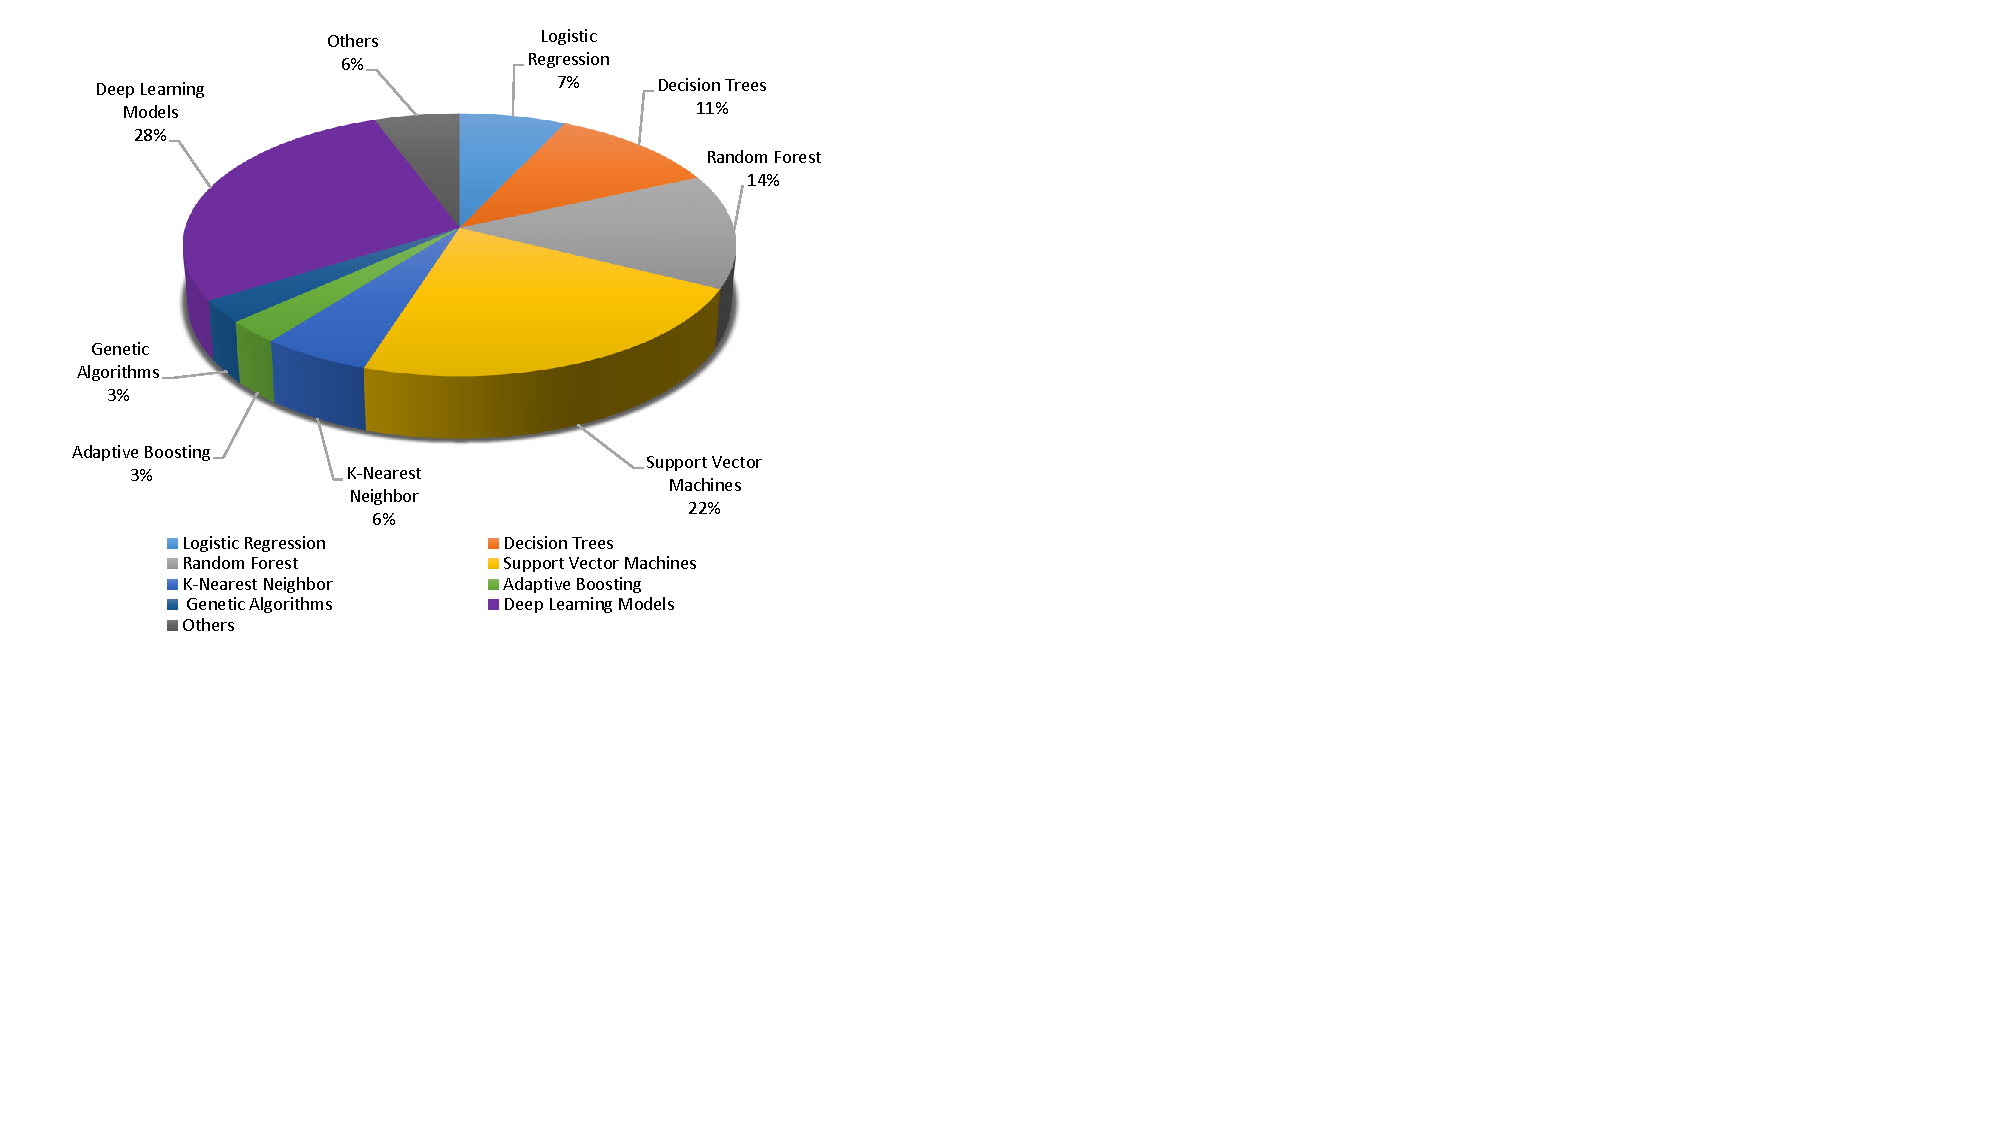
\includegraphics[width=0.55\linewidth]{PROYECTO/imgs/ModelosUsados}
	\end{figure}
\end{frame}

%----------------FRAME--------------------------------------------------------------
\begin{frame}
	\frametitle{Objetivos}
	\begin{alertblock} {Resultado}
		\justifying
		Para realizar el entrenamiento de los modelos de Machine Learning seleccionados, se utilizó el data set  de cáncer de mama, elaborado por la Universidad de Wisconsin y se utilizó la librería Scikit-Learn para el  procesamiento de datos  y el posterior entrenamiento de dichos modelos. 
	\end{alertblock}
\end{frame}

%----------------FRAME--------------------------------------------------------------
\begin{frame}
	\frametitle{Objetivos}
	\begin{block}{Objetivos Especificos}\justifying
		Realizar un análisis comparativo de la precisión de los modelos existentes utilizados en el diagnostico de cáncer de mama.	
	\end{block}
	
	\begin{alertblock}{Resultado}
		\justifying	
		La determinación de la precisión de los modelos es expresada como la relación entre los diagnósticos realizados correctamente y el número total de diagnósticos. 
	\end{alertblock}
	
	\begin{table}[ht]
		\begin{center}	
			\begin{tabular}{lc}
				\hline
				\rowcolor[HTML]{DADADA} 
				\multicolumn{1}{c}{\cellcolor[HTML]{DADADA}\textbf{Modelo}} & \textbf{Presición} \\ \hline
				Decision Trees                                              & 1.0                \\ \hline
				Random Forest                                               & 0.9953             \\ \hline
				Support Vector Machines(SVM)                                & 0.9647             \\ \hline
				Logistic Regression                                         & 0.9600             \\ \hline
				Gaussian Naive Bayes                                        & 0.9507             \\ \hline
				K-Nearest Neighbor (KNN)                                    & 0.9413             \\ \hline
			\end{tabular}
		\end{center}
	\end{table}
\end{frame}


%----------------FRAME--------------------------------------------------------------
\begin{frame}
	\frametitle{Objetivos}
	\begin{block}{Objetivos Especificos}\justifying
	Elaborar un aplicativo que sea capaz de diagnosticar el padecimiento de cáncer de mama de un paciente en particular. 
	\end{block}
	
	\begin{alertblock}{Resultado}
		\justifying	
		Implementación de la aplicación web llamada BreastApp V1.0 la cual está conformada por dos componentes: El Back-End de la aplicación el cual fue realizado en Python y el Front-End de la aplicación el cual fue realizado en Angular.Esta aplicación brinda  un dictamen del padecimiento de cáncer de mama soportado en datos y gráficas proporcionados por los modelos de Machine Learning utilizados.
	\end{alertblock}
\end{frame}
%----------------FRAME--------------------------------------------------------------
\begin{frame}
	\frametitle{Desarrollo de la Investigación}
	
	\justifying
	\begin{block}{Recolección de datos}\justifying
		En la investigación se identificaron nueve características evaluadas visualmente de una muestra obtenida por el método de aspiración por aguja fina (FNA)que se consideraron relevantes para el diagnóstico.El conjunto de datos resultante es conocido como el Data-Set de cáncer de mama de Wisconsin\cite{b2}.
	\end{block}
	\begin{figure}[h!]
		\centering
		\includegraphics[width=0.4\linewidth]{PROYECTO/imgs/fnaTest}
	\end{figure}
\end{frame}

%----------------FRAME--------------------------------------------------------------
\begin{frame}
	\frametitle{Desarrollo de la Investigación}
	\begin{block}{Verificación de datos}\justifying
		La verificación de los datos extraídos por medio de la muestra FNA y la veracidad del Data-Set  de cáncer de mama de Wisconsin se realiza con base a los resultados  del proceso realizado por el software conocido como Xcyt.Este sistema ha diagnosticado correctamente 176 nuevos pacientes consecutivos (119 benignos, 57 malignos)\cite{b3}.
	\end{block}
	\begin{figure}[h!]
		\centering
		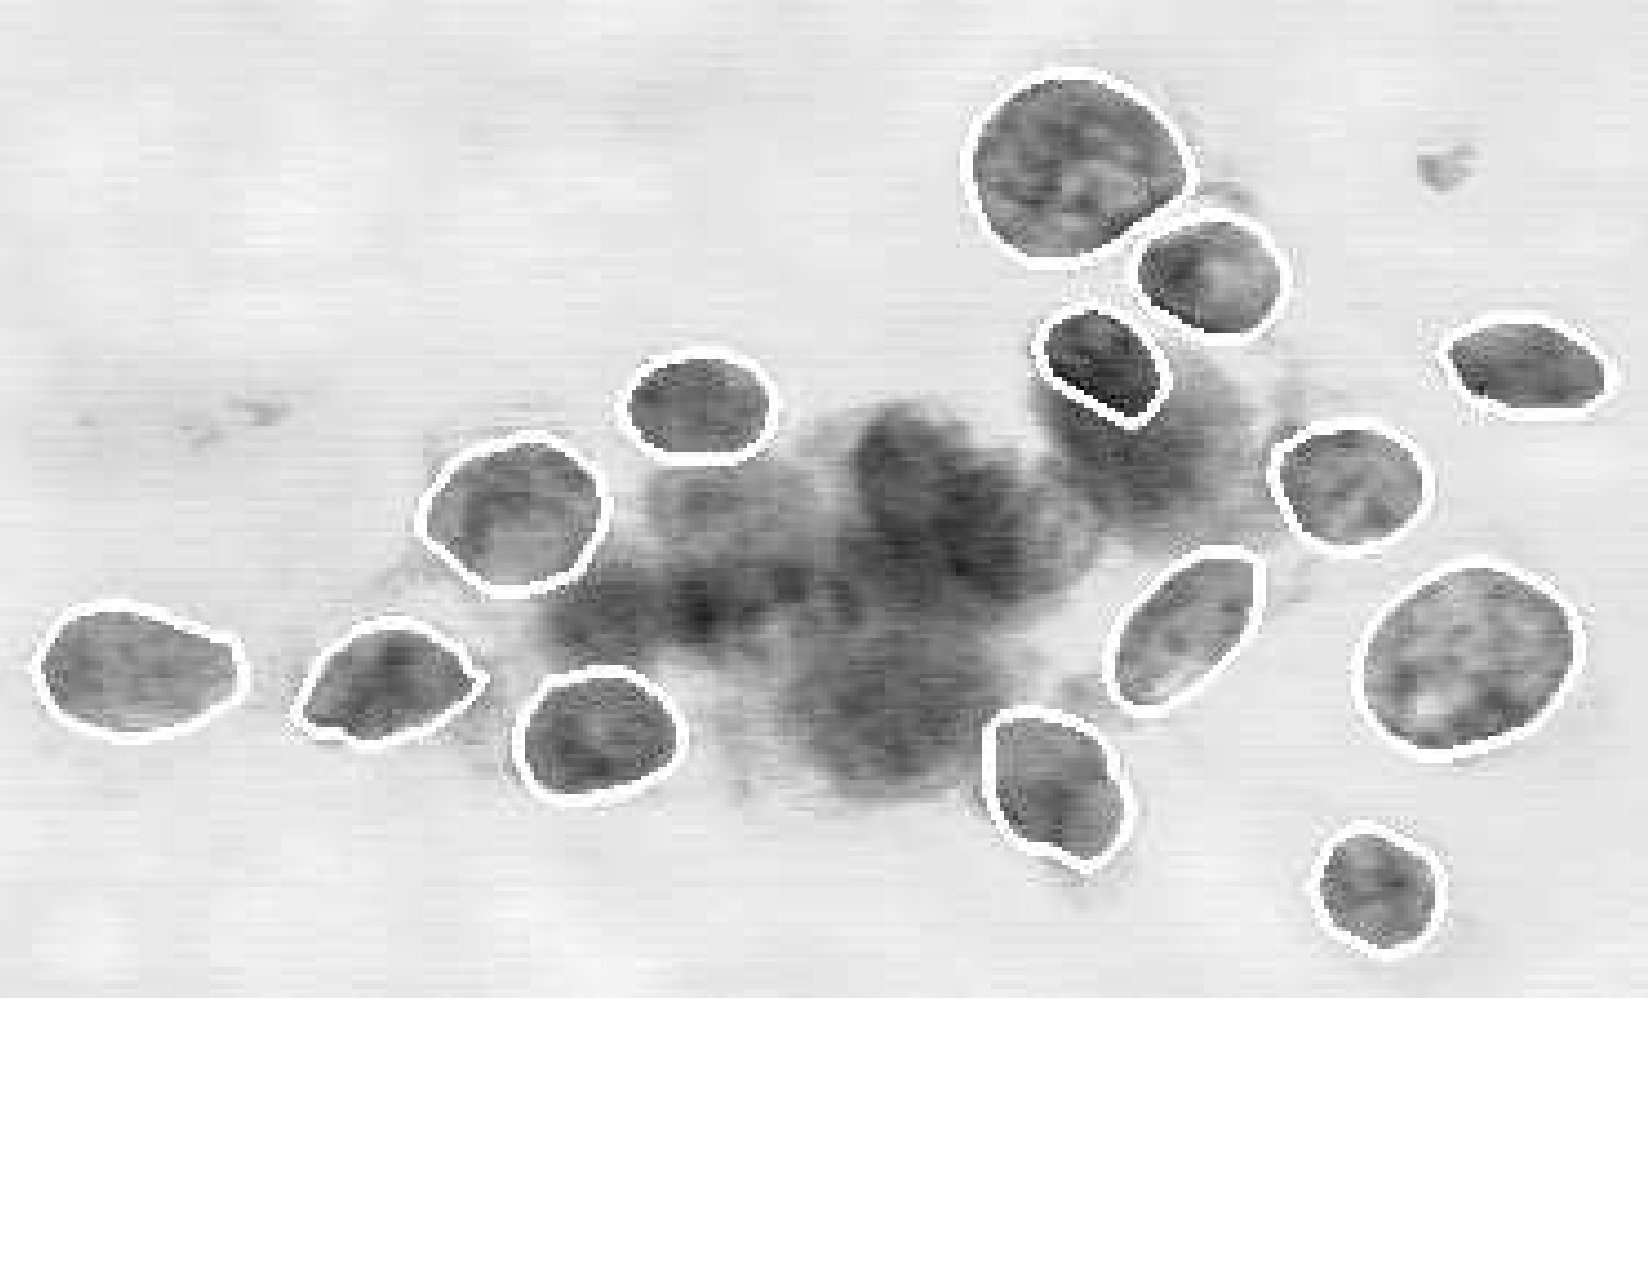
\includegraphics[width=0.5\linewidth]{PROYECTO/imgs/fna}
	\end{figure}
\end{frame}

%----------------FRAME--------------------------------------------------------------
\begin{frame}
	\frametitle{Desarrollo de la Investigación}
	\begin{block}{Clasificación de datos}\justifying
		El Sistema de enfoque de visión por computadora extrae diez características diferentes de los límites (snakes) de los núcleos celulares de la muestra FNA.  Las características extraídas son:
		\textit{Radius, Perimeter, Area, Texture, Smoothness, Concavity, Concave Points, Symmetry, Compactness y Fractal Dimension} \cite{b3}.
	\end{block}
	\begin{figure}[!htb]
		\minipage{0.24\textwidth}
		
\includegraphics[width=1\linewidth]{PROYECTO/imgs/FnaClassification/Concavity}
		\endminipage\hfill
		\minipage{0.24\textwidth}
		
\includegraphics[width=1\linewidth]{PROYECTO/imgs/FnaClassification/FractalDimension}
		\endminipage\hfill
		\minipage{0.24\textwidth}
		
\includegraphics[width=1\linewidth]{PROYECTO/imgs/FnaClassification/Smothness}
		\endminipage\hfill
		\minipage{0.24\textwidth}%
	    
\includegraphics[width=1\linewidth]{PROYECTO/imgs/FnaClassification/Symmetry}
		\endminipage
	\end{figure}
\end{frame}

%----------------FRAME--------------------------------------------------------------
\begin{frame}
	\frametitle{Desarrollo de la Investigación}
	\begin{block}{Limpieza de datos}\justifying
		Para el correcto entrenamiento de los modelos con el Data-Set es relevante tener alta calidad  en los datos, para ello fue necesario la corrección de los errores de los mismos para el posterior procesamiento con  los algoritmos de Machine Learning.
	\end{block}
	
	\begin{block}{Formateo de datos}\justifying
		Para la comprobación de los tipos de datos del  Data-Set de cáncer de mama de la Universidad de Wisconsin se utilizo  la librería \textit{Pandas} la cual cuenta con la propiedad \textit{dtypes} que describe los tipos de datos de las variables de dicho Data-Set.
	\end{block}
\end{frame}


%----------------FRAME--------------------------------------------------------------
\begin{frame}
	\frametitle{Desarrollo de la Investigación}
	\begin{block}{Comprobación de datos faltantes}\justifying
		Para la comprobación de datos faltantes se utilizo la librería \textit{Pandas} la cual cuenta con la función \textit{isna()} que valida si las variables contienen valores \textit{Nulos(Nan)}. En este caso en especifico el Data-Set de cáncer de mama de la Universidad de Wisconsin no contiene ningún valor nulo.
	\end{block}
	\begin{block}{Eliminación de datos Innecesarios}\justifying
		Para la eliminación de datos innecesarios se utilizo a la librería \textit{Pandas} la cual cuenta con la función \textit{dropna()} con la cual se eliminaron datos que no aportaban informacion necesaria para el diagnostico.
	\end{block}
\end{frame}
%----------------FRAME--------------------------------------------------------------
\begin{frame}
	\frametitle{Desarrollo de la Investigación}
	\begin{block}{Procesamiento de los Datos}\justifying
		El Data-Set se encuentran en formato .csv que es leído y cargado en memoria con la ayuda de las librerías de Python para luego ser asignado a una variable que hace que la información sea manejable. Dentro del Data-Set se encuentran  357 registros  de personas con tumores diagnosticados  como Benignos  y 212 como Malignos, esta información fue utilizada para entrenar y testear el modelo \cite{b4}.
	\end{block}
	\begin{figure}[h!]
	\centering
	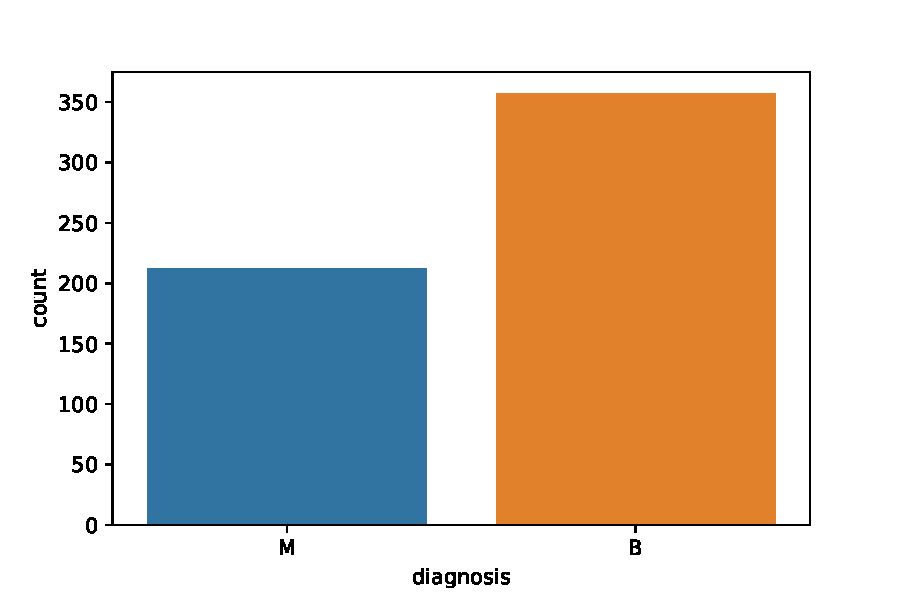
\includegraphics[width=0.5\linewidth]{PROYECTO/imgs/output}
	\end{figure}

\end{frame}

%----------------FRAME--------------------------------------------------------------
\begin{frame}
	\frametitle{Desarrollo de la Investigación}
	\begin{block}{Modelos de Machine Learning}\justifying
		Para la implementación técnica se utilizo la librería para \textit{Python} llamada \textit{Scikit-Learn} la cual contiene un conjunto de funciones para aplicar dichos modelos. Los modelos  seleccionados fueron: \textit{Logistic Regression}, \textit{Decision Trees},\textit{Gaussian Naive Bayes},\textit{K-Nearest Neighbors(KNN)},\textit{Random Forest},y \textit{Support Vector Machines(SVM)}\cite{b4}.
	\end{block}
\end{frame}

%----------------FRAME--------------------------------------------------------------
\begin{frame}
	\frametitle{Desarrollo de la Investigación}
	\begin{figure}[!htb]
		\minipage{0.32\textwidth}
		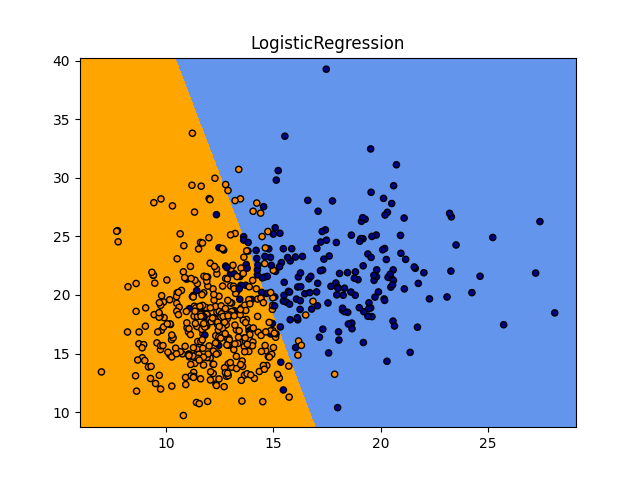
\includegraphics[width=1\linewidth]{PROYECTO/imgs/metodos/1_LogisticRegression}
		\endminipage\hfill
		\minipage{0.32\textwidth}
		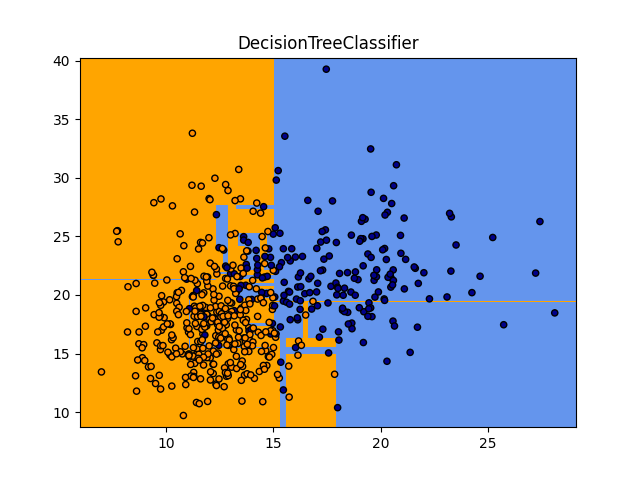
\includegraphics[width=1\linewidth]{PROYECTO/imgs/metodos/2_DecisionTreeClassifier}
		\endminipage\hfill
		\minipage{0.32\textwidth}
		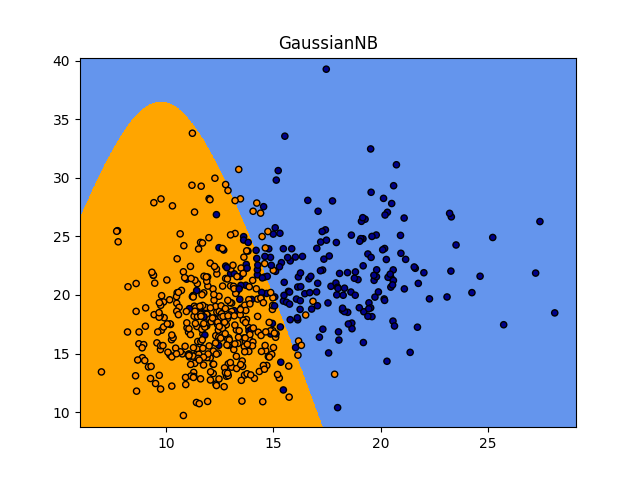
\includegraphics[width=1\linewidth]{PROYECTO/imgs/metodos/3_GaussianNB}
		\endminipage\hfill
	\end{figure}
	
	\begin{figure}[!htb]
		\minipage{0.32\textwidth}
		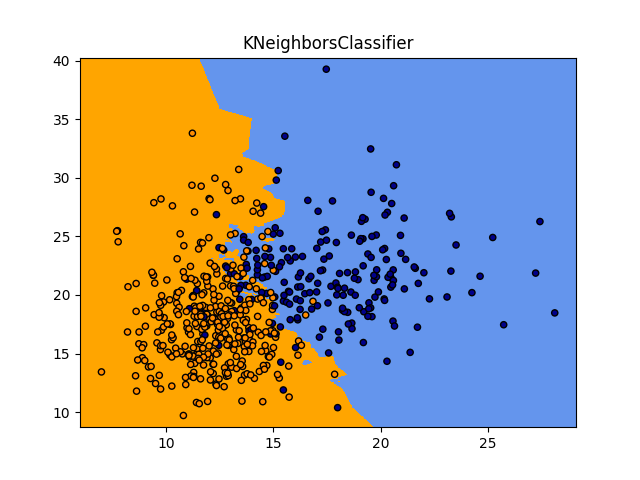
\includegraphics[width=1\linewidth]{PROYECTO/imgs/metodos/4_KNeighborsClassifier}
		\endminipage\hfill
		\minipage{0.32\textwidth}
		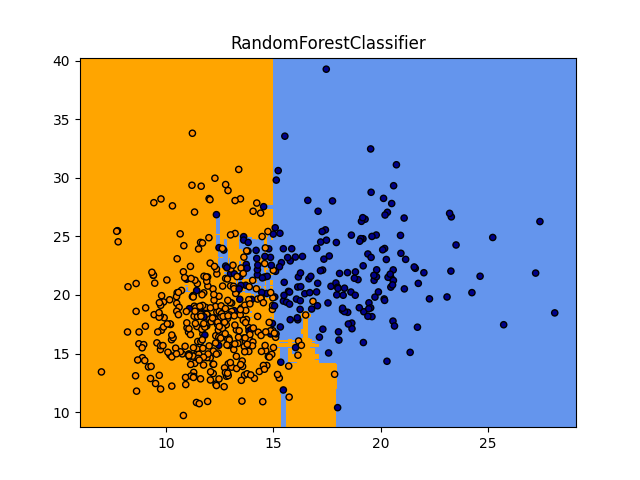
\includegraphics[width=1\linewidth]{PROYECTO/imgs/metodos/5_RandomForestClassifier}
		\endminipage\hfill
		\minipage{0.32\textwidth}
		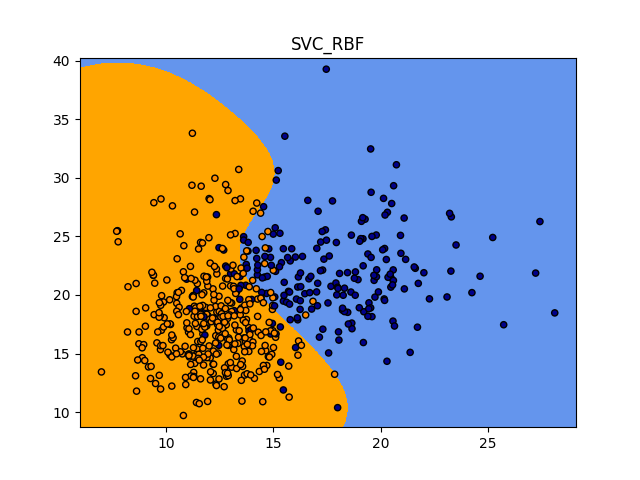
\includegraphics[width=1\linewidth]{PROYECTO/imgs/metodos/6_SupportVectorMachinesRBF}
		\endminipage\hfill
	\end{figure}
	
\end{frame}

%----------------FRAME--------------------------------------------------------------
\begin{frame}
	\frametitle{Conclusiones}
	\begin{itemize}\justifying
	\item Con respecto a los modelos de Machine Learning utilizados por diversos investigadores para predecir el Cáncer de mama se puede evidenciar que el algoritmo más utilizado es el Support Vector Machines (SVM), pero al realizar la comparación con los resultados obtenidos de la precisión de los métodos de Machine Learning observados anteriormente, el algoritmo Decision Trees es el que mejor resultado tiene, con una exactitud del 100\%, esto quiere decir que clasifico correctamente el total de las muestras. Por lo tanto según la investigación realizada  se concluye que si se va a diagnosticar el Cáncer de mama los modelos más indicados para hacerlo son el Support Vector Machines(SVM) y Decision Trees.
	\end{itemize}
\end{frame}
%----------------FRAME--------------------------------------------------------------
\begin{frame}
	\frametitle{Conclusiones}
	\begin{itemize}\justifying
		\item Según el análisis realizado con base en el diagrama de calor conformado por la correlación de las variables del Data-Set de la Universidad de Wisconsin se puede evidenciar que  las variables \textit{concave\_points\_worst} y \textit{area\_worst} generan información relevante en la realización del diagnóstico de Cáncer de mama debido a  que expresan  una deformidad mayor de los núcleos celulares encontrados en las masas mamarias extraídas por el método de Aspiración con Aguja Fina(FNA).
	\end{itemize}
\end{frame}
%----------------FRAME--------------------------------------------------------------
\begin{frame}
	\frametitle{Aportes Originales}
	\begin{itemize}\justifying
		\item Implementación de una capa de servicios REST basada modelos de Machine Learning para el diagnóstico de Cáncer de mama que podría ser utilizada en diferentes ámbitos en la detección y el diagnóstico de dicho Cáncer.
		
		\item Diseño y Arquitectura de un aplicativo web enfocado en el uso de modelos de Machine Learning aplicados en la rama de la Medicina especializada en Oncología.
	\end{itemize}
\end{frame}

%----------------FRAME--------------------------------------------------------------
\begin{frame}
	\frametitle{Trabajos Futuros}
	\begin{itemize}\justifying
		\item Creación de una aplicación web llamada OncoAnalysisApp la cual permita el diagnóstico de cualquier tipo de Cáncer teniendo como entrada Data-Sets obtenidos por diversos métodos médicos.
		\item Creación de una aplicación que permita el análisis de imágenes y que diagnostique el padecimiento de Cáncer de mama con base a los modelos de Deep-Learning existentes.
		\item Creación de una aplicación que permita crear nuevos Data-Set dinámicamente según parámetros proporcionados por el usuario. 
	\end{itemize}
\end{frame}



%----------------FRAME-------------------------------------------------------------
\begin{frame}
	\frametitle{Bibliografía}	
	\bibliographystyle{unsrt}
	\bibliography{REFERENCIAS/articulos}
\end{frame}


\end{document}